% \graphicspath{{thesis-source/}{ch3_oct_localization/}{Figures/}}
\section{Introduction}
\label{sec:oct_introduction}
\autoindex{Age-Related Macular Degeneration} (AMD) and \autoindex{Diabetic Retinopathy} (DR) are two of the most common eye diseases, with over 300 million patients at risk of losing sight worldwide~\sidecite{Bourne2017}. To diagnose and manage these chronic retinal conditions, 30 million \autoindex{Optical Coherence Tomography} (OCT) are taken each year, yielding micron-resolution 3D volumes of the retina in a routine, fast, and noninvasive way. OCT has become a crucial instrument for establishing patient treatments and a dependable tool to validate the efficacy of novel therapeutic approaches to treat eye diseases.

In this context, \autoindex{intraretinal fluid} (IRF) and \autoindex{subretinal fluid} (SRF) are well-established markers that are directly linked to both AMD and DR~\sidecite{Phadikar2017,zur2017}. Their identification and localization within a set of concentric rings, known as the \autoindex{Early Treatment Diabetic Retinopathy Study} (ETDRS) rings~\sidecite{Domalpally2018}, is critical for disease assessments\footnote{See~\cref{fig:etdrs_rings}}, as the different ETDRS ring regions are linked to different visual function levels (\ie,~higher risk of vision loss when markers are in the central 1mm ring and lower risk when in the 6mm ring). Driven by this clinical need, numerous methods have been proposed to automate the process of identifying markers such as IRF and SRF~\sidecite{Trucco2020}, and the work here follows this research direction too.
%\begin{figure*}[t]
%%\centering
%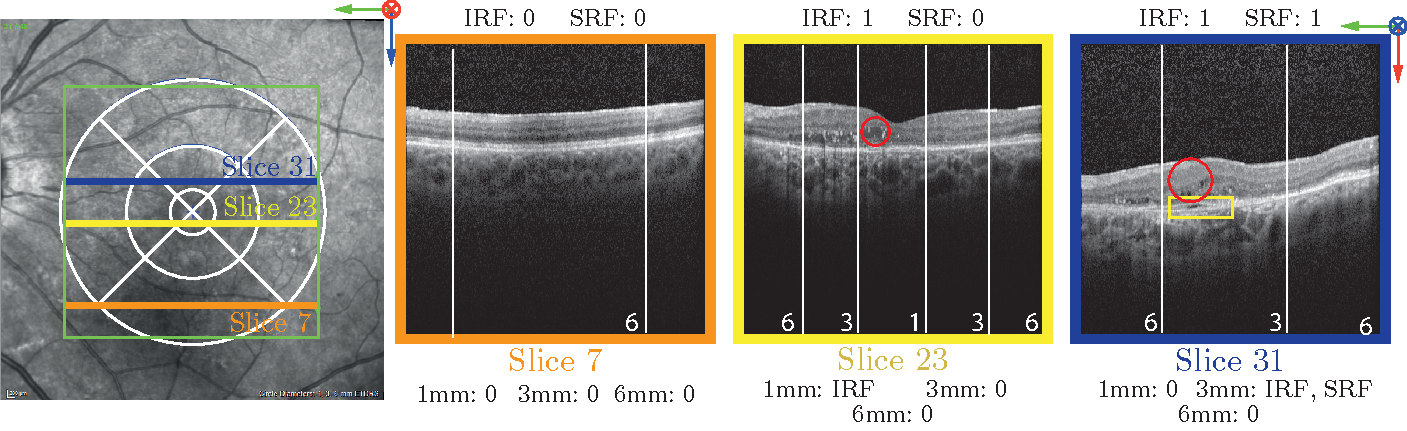
\includegraphics[width=\textwidth]{Figures/fig1_SLO.pdf}
%\sidecaption{Left: View of the retina, the OCT volume (green square) and the ETDRS rings (white) which are virtually placed on the surface of the retina. Right: Three 2D OCT slices at different positions of the OCT volume.
%Red circles indicate IRF biological marker and the yellow rectangle indicates SRF (Figure best seen in color).
%}
%\label{fig:etdrs_rings}
%\end{figure*}

%\plainwidefig{1}{Figures/fig1_SLO.pdf}{Left: View of the retina, the OCT volume (green square), and the ETDRS rings (white) which are virtually placed on the surface of the retina. Right: Three 2D OCT slices at different positions of the OCT volume. Red circles indicate IRF biological marker and the yellow rectangle indicates SRF (Figure best seen in color).}{fig:etdrs_rings}


Previous methods have included IRF and SRF detection and segmentation models~\sidecite{DeZanet2020,Lee2018,Liefers2021,Yim2020}. While segmentation models have the advantage of quantifying IRF and SRF regions, they often require a large amount of manually annotated segmentation labels for optimal performance.\index{weakly supervised semantic segmentation} To counteract this issue, some works use weak annotations, such as slice level labels, retinal layer positioning, and foveal distance, to achieve voxel-wise segmentations~\sidecite{Schlegl}. Weak annotations offer a wide range of possibilities, and therefore others have studied the use of bounding boxes to develop positive-aware lesion detection networks~\sidecite{Fan2020}. More relevant to our work, some methods only use slice-level annotations~\sidecite{ma2020}. Here, Ma et al. presented a weakly-supervised segmentation method for Geographic Atrophy (GA) lesions in Spectral Domain OCT images.  The method first segments the retinal pigment epithelium and then extracts a class activation map from multi-scale features. The final en-face binary segmentation of GA is obtained by refining the map with Conditional Random Fields, utilizing only slice-level labels with binary information about the presence of GA.

\plainwidefig[t]{1}{Figures/fig1_SLO.pdf}{Left: View of the retina, the OCT volume (green square), and the ETDRS rings (white) which are virtually placed on the surface of the retina. Right: Three 2D OCT slices at different positions of the OCT volume. Red circles indicate IRF biological marker and the yellow rectangle indicates SRF (Figure best seen in color).}{fig:etdrs_rings}

Similarly, ensembles of Convolutional Neural Networks (CNNs) have been proposed to detect IRF and SRF in individual slices using only binary annotations on a slice level~\sidecite{Kurmann2019,Kurmann2019a}. However, by removing the need for segmentation annotations, these methods cannot provide any location information.  In this work, we propose a novel weakly supervised deep learning framework that overcomes these limitations and enables the detection and localization of 2D OCT markets in ETDRS rings without requiring costly location information during training. Specifically, our method uses binary annotations of marker presence in OCT slices during training and infers marker presence and marker location in ETDRS rings during test time. To do this, we introduce a pooling strategy where we treat our network's convolutional feature maps in such a way as to preserve spatial relations that can be partially pooled for coarse localization. This is combined with a novel loss function that enforces geometrically and biologically plausible solutions. This allows ring assignment to be performed as a post-processing step independent of the training phase. Our experiments demonstrate that our method predicts the location of markers in ETDRS rings with high accuracy, thereby significantly outperforming previous methods that use the same amount of training information. 